\chapter{Results}\label{chap:Results}

\section{Exploratory Data Analysis}\label{sec:Exploratory_Data_Analysis}

\subsection{HMDA Data}\label{subsec:HMDA_EDA}

After all preparation steps detailed in \textbf{chapter \ref{subsec:HMDA_Data}}, the dataset contained \textit{851,936} observations and \textit{9} features (including the target variable, \textit{loan\_granted}). 

\textbf{EDA of the Target Variable}

The target variable, \textit{loan\_granted}, is binary (\textit{Granted} or \textit{Not Granted}) and imbalanced, with \textit{57.9\%} of all loans being granted. 
There were no missing values. The distribution of the target variable can be seen in \textbf{figure \ref{fig:CHXX_Target_Variable_Distribution}}.

\begin{figure}[h]
    \centering
    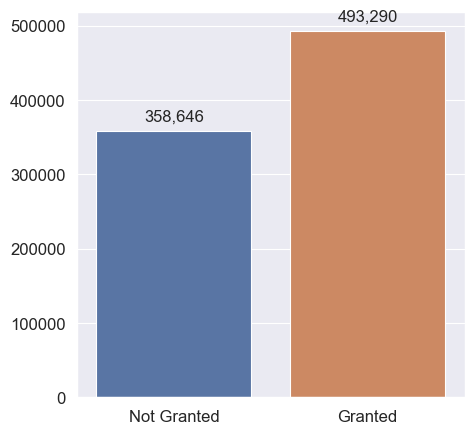
\includegraphics[width=0.6\textwidth]{images/CHXX_Target_Variable_Distribution.png}
    \caption{HMDA: Distribution of the Target Variable}
    \medskip
    \small
    The target variable is imbalanced, with 57.9\% (493,290) of all loans being granted.
    \label{fig:CHXX_Target_Variable_Distribution}
\end{figure}

Analyzing the correlation of the target variable with the categorical and numerical features showed that the \textit{debt\_to\_income\_ratio} feature has the highest correlation (moderate negative correlation of \textbf{-0.61}) with the target variable, while the other features show only weak correlations. 
The correlation of the target variable with the numerical and categorical features can be seen in \textbf{figure \ref{fig:CHXX_Target_Correlation_Categorical}} and \textbf{figure \ref{fig:CHXX_Target_Correlation_Numerical}}, respectively.

\begin{figure}[hbt!]
    \centering
    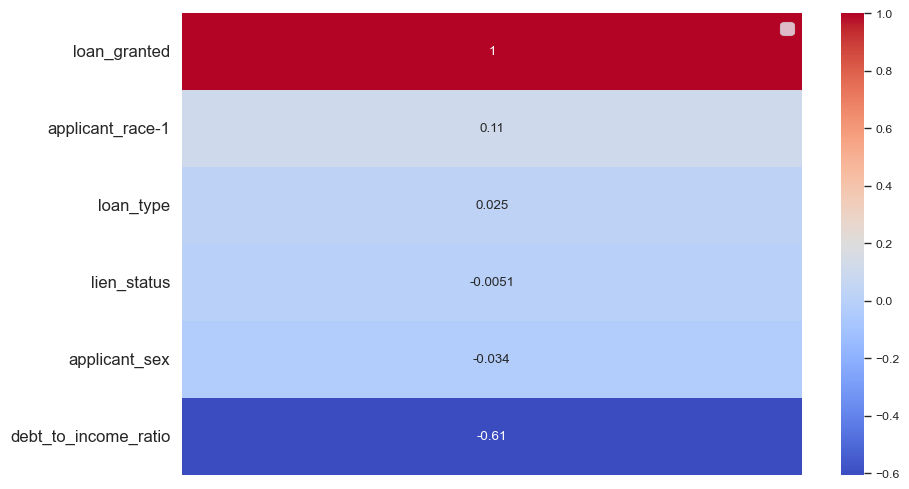
\includegraphics[width=1\textwidth]{images/CHXX_Target_Correlation_Categorical.png}
    \caption{HMDA: Correlation of the Target Variable with Categorical Features}
    \medskip
    \small
    While there are only weak correlations between \textit{loan\_granted} and \textit{applicant\_race-1, loan\_type, lien\_status}, and \textit{applicant\_sex}, there is a moderate negative correlation of \textbf{-0.61} between \textit{loan\_granted} and \textit{debt\_to\_income\_ratio}.
    \label{fig:CHXX_Target_Correlation_Categorical}
\end{figure}

\begin{figure}[hbt!]
    \centering
    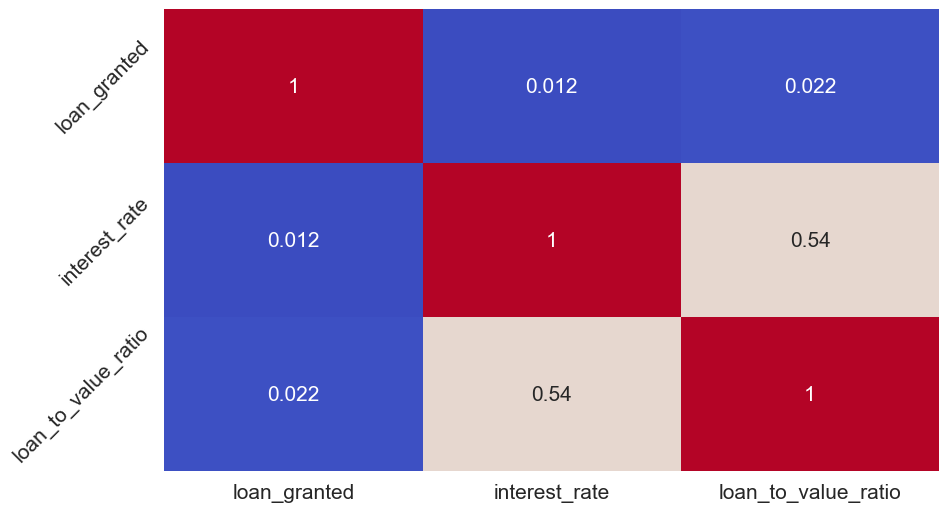
\includegraphics[width=1\textwidth]{images/CHXX_Target_Correlation_Numerical.png}
    \caption{HMDA: Correlation Between the Numerical Features}
    \medskip
    \small
    While both numerical features are only weakly correlated with \textit{loan\_granted}, there is a moderate positive correlation of \textbf{0.54} inbetween them.
    \label{fig:CHXX_Target_Correlation_Numerical}
\end{figure}

% \subsection{Data Overview}\label{subsec:Data_Overview}

\textbf{EDA of the Features}

The processed dataset contained two \textit{numerical} features: \textbf{interest\_rate} and \textbf{loan\_to\_value\_ratio}.
% Their distributions can be seen in \textbf{Figure \ref{fig:CHXX_Numerical_Distributions_1}} and \textbf{Figure \ref{fig:CHXX_Numerical_Distributions_2}}.
Their distributions can be seen in \textbf{figure \ref{fig:CHXX_Numerical_Distributions_2}}.
% Both are positively correlated with each other with a correlation coefficient of \textit{0.54}.

%\begin{figure}[h]
%    \centering
%    \caption{Boxplots of the Numerical Features}
%    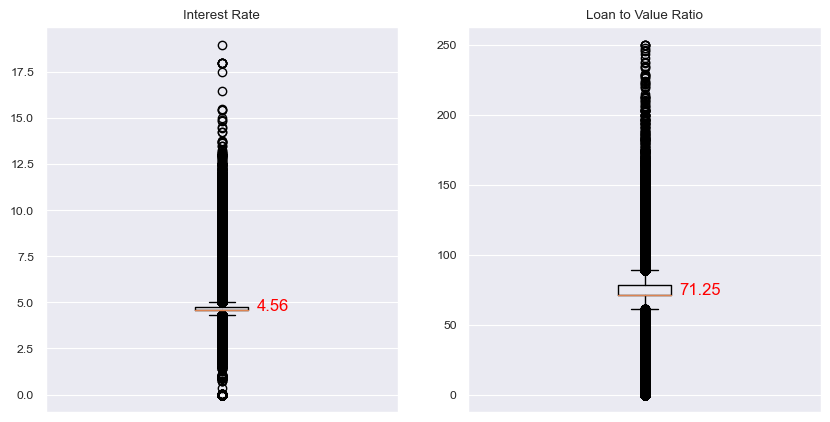
\includegraphics[width=0.85\textwidth]{CHXX_Numerical_Distributions_1.png}
%    \caption*{The results of the KNNImputer applying mean (annotated in red) values for all missing values show clearly here by the narrow quartiles.}
%    \label{fig:CHXX_Numerical_Distributions_1}
%\end{figure}

\begin{figure}[h]
    \centering
    \begin{minipage}{0.5\textwidth}
        \centering
        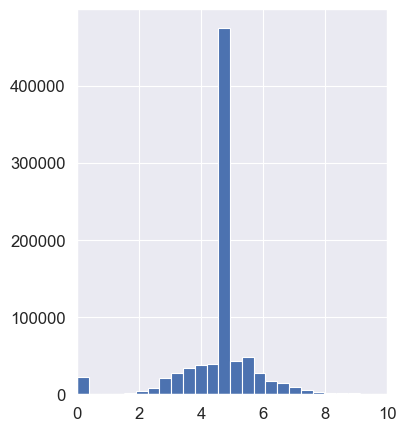
\includegraphics[width=\textwidth]{images/CHXX_Numerical_Distributions_2_IR.png}
        \small
        Interest Rate
    \end{minipage}\hfill
    \begin{minipage}{0.5\textwidth}
        \centering
        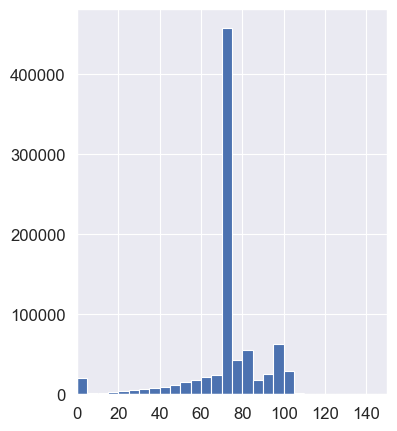
\includegraphics[width=\textwidth]{images/CHXX_Numerical_Distributions_2_LTVR.png}
        \small
        Loan to Value Ratio
    \end{minipage}    
    \caption{HMDA: Histograms of the Numerical Features}
    \medskip
    \small
    The results of the KNNImputer applying mean (\textit{4.56\%} for the interest rate and \textit{71.24\%} for the Loan to Value Ratio) values for the loan to value ratio values for all missing values show clearly here by the high amount of values at the mean.
    \label{fig:CHXX_Numerical_Distributions_2}
\end{figure}

Exploratory data analysis of the categorical variables showed that the majority of loan applicants are \textbf{White} (65\%) and \textbf{Male} (85\%), resulting in 57\% of all applicants being both White and Male.
Most loans applied for are \textbf{Conventional} (82\%) and \textbf{First Lien} (86\%).
Aside from missingness in the \textit{debt\_to\_income\_ratio} feature, which alone accounts for 26\% of all values, the data in this feature are roughly normally distributed, with the mode being 14\% of values in the \textbf{36\%-41\%} range. 
The distributions of the categorical variables can be seen in \textbf{figure \ref{fig:HMDA_Categorical_Features_Distributions}}.

\begin{figure}[h]
    \centering
    \begin{minipage}{0.5\textwidth}
        \centering
        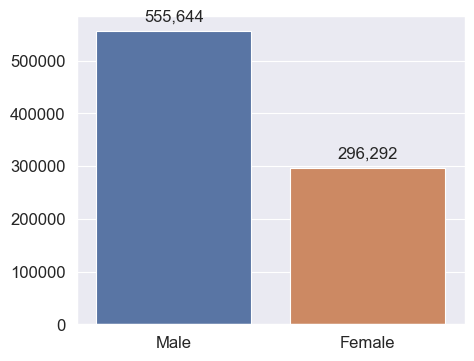
\includegraphics[width=\textwidth]{images/HMDA_features/HMDA_features_sex.png}
        \small
        Applicant Sex
    \end{minipage}\hfill
    \begin{minipage}{0.5\textwidth}
        \centering
        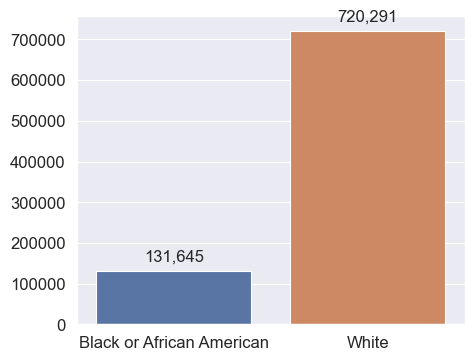
\includegraphics[width=\textwidth]{images/HMDA_features/HMDA_features_race.png}
        \small
        Applicant Race
    \end{minipage}
    
%    \vspace{1em} 

    \begin{minipage}{0.5\textwidth}
        \centering
        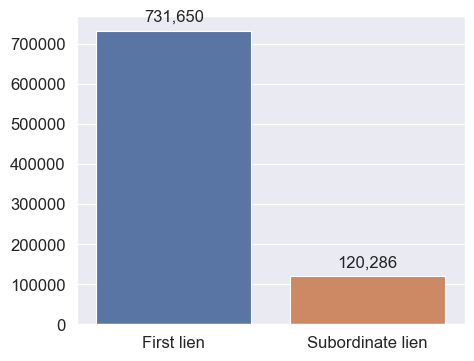
\includegraphics[width=\textwidth]{images/HMDA_features/HMDA_features_lien.png}
        \small
        Lien Status
    \end{minipage}\hfill
    \begin{minipage}{0.5\textwidth}
        \centering
        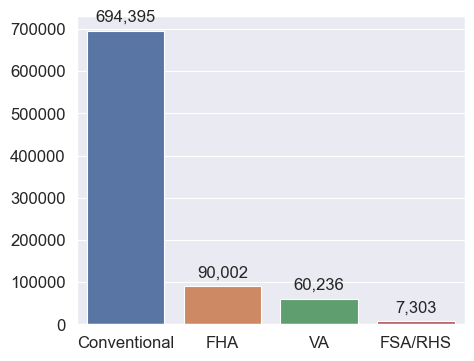
\includegraphics[width=\textwidth]{images/HMDA_features/HMDA_features_type.png} 
        \small
        Loan Type
    \end{minipage}

%    \vspace{1em}

    \centering
    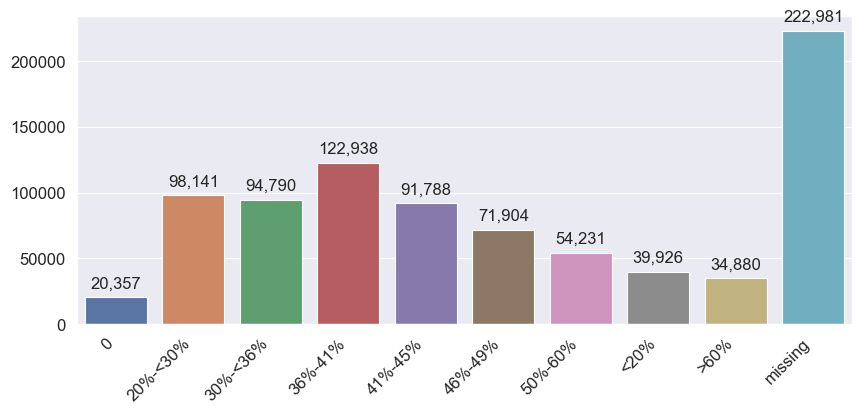
\includegraphics[width=\textwidth]{images/HMDA_features/HMDA_features_dtir.png}
    \small
    Debt to Income Ratio

    \caption{HMDA: Distributions of the Categorical Features}
    \label{fig:HMDA_Categorical_Features_Distributions}
    \medskip
    \small
    The majority of loan applicants are \textit{Male} and \textit{White}. Most loans applied for are \textit{Conventional} and \textit{First Lien}. The \textit{debt\_to\_income\_ratio} feature is (apart from the missing values) roughly normally distributed, with the mode being 14\% of values in the \textbf{36\%-41\%} range.

\end{figure}

% \subsection{Fairness}\label{subsec:Fairness}

\textbf{EDA of Fairness Aspects}

Following the scope of this thesis specified in \textbf{chapter \ref{ch:Introduction}}, a special focus needs to be put  on fairness, specifically equality with regards to the protected attribute(s).
This potential unfairness in the underlying data can be identified from assessing the distribution of the target variable across different groups.
\textbf{Figure \ref{fig:CHXX_Loan_Grant_By_Protected_Attribute}} shows the amount of (not) granted loans per race and by sex, the probabilities of being granted a loan across these groups can be found in \textbf{table \ref{tab:loan_granting}}.\@

\begin{figure}[h]
    \centering
    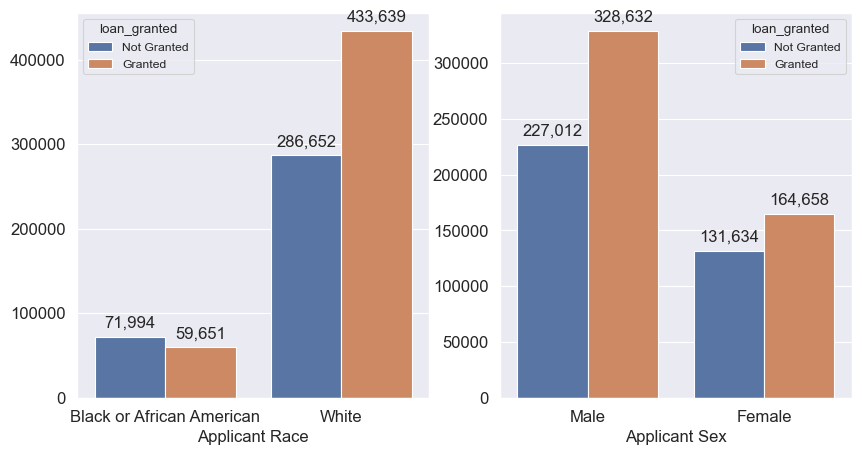
\includegraphics[width=0.85\textwidth]{CHXX_Loan_Grant_By_Protected_Attribute.png}
    \caption{Loan Grant by Protected Attribute}
    \caption*{Discrimination by race is apparent in the data, as the amount of granted loans differs significantly}
    \label{fig:CHXX_Loan_Grant_By_Protected_Attribute}
\end{figure}

\begin{table}[htbp]
    \centering
      \begin{tabular}{lcc}
      \toprule
      \textbf{Applicant Race} & \textbf{Applicant Sex} & \textbf{Loan Granted (\%)} \\
      \midrule
      Black or African American & Male    & 46.4 \\
            & Female  & 44.1 \\
      White & Male    & 60.9 \\
            & Female  & 58.8 \\
      \bottomrule
      \end{tabular}
      \caption{Loan Granting Statistics by Applicant Race and Sex}
      \caption*{Analyzing the differences in percentages of loans being granted among race and sex of applicants shows differences in the underlying data: Regardless of their gender, Black or African American applicants are less likely to be granted a loan than White applicants.}
    \label{tab:loan_granting}%
\end{table}%

Even though the focus of the analysis is on the \textit{applicant\_race-1} attribute, \textit{applicant\_sex} has been included as a second discriminating factor, as it also constitutes a protected attribute.
Inspection of the results depicted here did however imply that the issue of racial equality is more pronounced than that of inequality between the sexes.
A chi-squared test of independence proved that assumption of underlying inequality between races in the data, as the p-value is \textit{<0.01} and therefore H0 (equality in granted loans) could be rejected at any significance level.
Utilizing the aforementioned \textbf{AIF360} package to assess the mean difference of granted loans between the races in the underlying data amounted to a \textit{14.9\%} difference.

\subsection{Enrichment Data}\label{subsec:Enrichment_Data}

As stated before, analyzing the geographical information provided in the enrichment dataset (see \textbf{chapter \ref{subsec:Explainability}}) was expected to provide additional insights into the fairness of the model.
A sign of potential discrimination in the data could be the correlation between race and potentially favorable outcomes, such as a higher percentage of granted loans or a lower poverty rate.
\textbf{Figure \ref{fig:Scatter_White_Applicants_Loan_Grant}} shows a scatterplot that relates the percentage of White applicants to the percentage of granted loans per county. It indicates that a higher percentage of white applicants per county does not only seem to be correlated with a higher percentage of these loans actually being granted, but also with a lower poverty rate on average.

\begin{figure}[h]
    \centering
    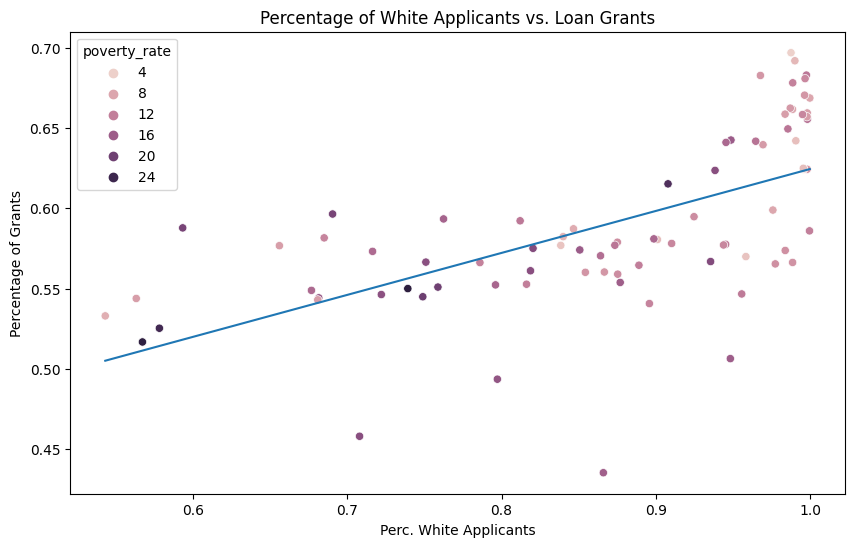
\includegraphics[width=0.85\textwidth]{images/CHXX_Perc_Grants_vs_Perc_White.png}
    \caption{Relationship between Applicant Race, Poverty Rate and Loan Grants}
    \caption*{Counties with predominantly White applicants do not only tend to have a lower poverty rate on average, but also see a higher percentage of loans being granted on average.}
    \label{fig:Scatter_White_Applicants_Loan_Grant}
\end{figure}

It should however be noted that the distributions within the enrichment data themselves are skewed by nature, as there are way higher numbers of White applicants in the data set and only few counties have a substantial number of predicted mortgage grants (see \textbf{figure \ref{fig:Enrichment_Data_EDA}}).

\begin{figure}[h]
    \centering
    \begin{minipage}{0.33\textwidth}
        \centering
        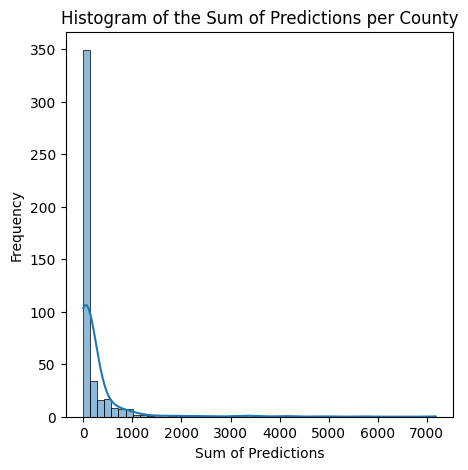
\includegraphics[width=\textwidth]{images/geo_enrich/predictions_per_county.png}
        \small
        Applications per County
    \end{minipage}\hfill
    \begin{minipage}{0.33\textwidth}
        \centering
        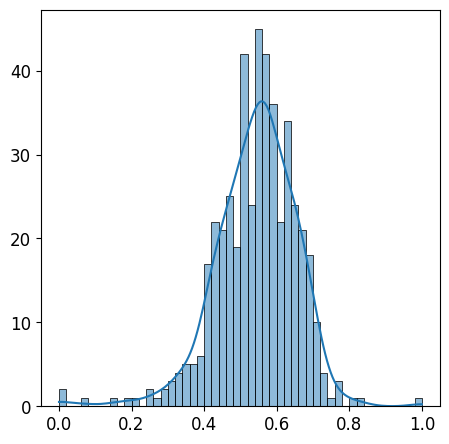
\includegraphics[width=\textwidth]{images/geo_enrich/perc_predictions.png}
        \small
        Percentage of Grants
    \end{minipage}\hfill
    \begin{minipage}{0.33\textwidth}
        \centering
        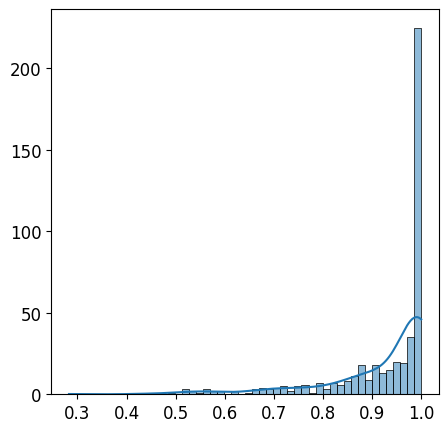
\includegraphics[width=\textwidth]{images/geo_enrich/white_per_county.png}
        \small
        Percentage of White Applicants
    \end{minipage}\hfill
    \caption{Enrichment Data EDA}
    \label{fig:Enrichment_Data_EDA}
    \medskip
    \small
    Analyzing the enrichment data shows that while the percentage of predictions per county appears to be normally distributed, the distributions of the percentage of White applicants and the percentage of predicted granted loans per county are skewed.
\end{figure}

%\section{Results}\label{sec:Results}      

As defined in \textbf{chapter \ref{subsec:Performance_Assessment}} and \textbf{chapter \ref{subsec:Fairness_Assessment}}, each outcome is assessed in terms of performance and fairness with two pre-defined metric sets. Additionally, the aspect of Explainability will be demonstrated examplarily for the initial model run.

\subsection{Initial Performance}\label{subsec:Initial_Performance}

The initial run serving as a benchmark was conducted training the neural network described in \textbf{chapter \ref{subsec:Model_Training_and_Prediction}} on the unadjusted training data (see \textbf{chapter \ref{subsec:HMDA_Data}}).

\textbf{Explainability}

As was intended in \textbf{chapter \ref{subsec:Explainability}}, three different Explainability algorithms were utilized to challenge each other's results and analyze overall patterns. \textbf{figure \ref{fig:SHAP_explanations}} and \textbf{figure \ref{fig:LIME_explanations}} show the individual explanations for the first 150 observations of the test set provided by SHAP and LIME, respectively. 
As already mentioned in \textbf{chapter \ref{subsec:Performance_Assessment}}, the model behaved somewhat different from the expectations: Imputation of missing values in the \textit{debt\_to\_income\_ratio} feature led to a significant decrease in both fairness and performance measures of the model.
Therefore, it must be assumed that missingness in itself is not completely at random and holds information (or that the imputation method via a random forest regressor is not suitable for this task).
While SHAP considers that missingness to be the most important influence on model predictions, LIME weighs the \textit{debt\_to\_income\_ratio} features higher in general.
None of the algorithms consider the protected attributes to be of high direct impact on the results.

\begin{figure}[h]
    \centering
    \begin{minipage}{0.5\textwidth}
        \centering
        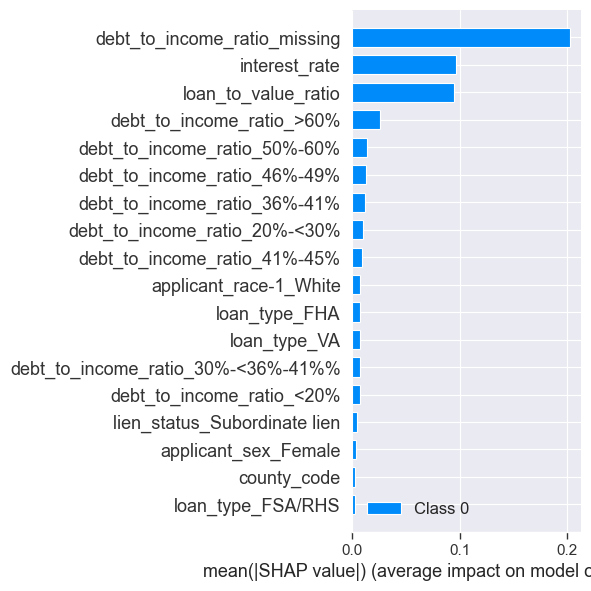
\includegraphics[width=\textwidth,height=5cm,keepaspectratio]{images/CHXX_UPDATE_SHAP_individual.png}
        \caption{SHAP individual explanations}
        \label{fig:SHAP_explanations}
    \end{minipage}\hfill
    \begin{minipage}{0.5\textwidth}
        \centering
        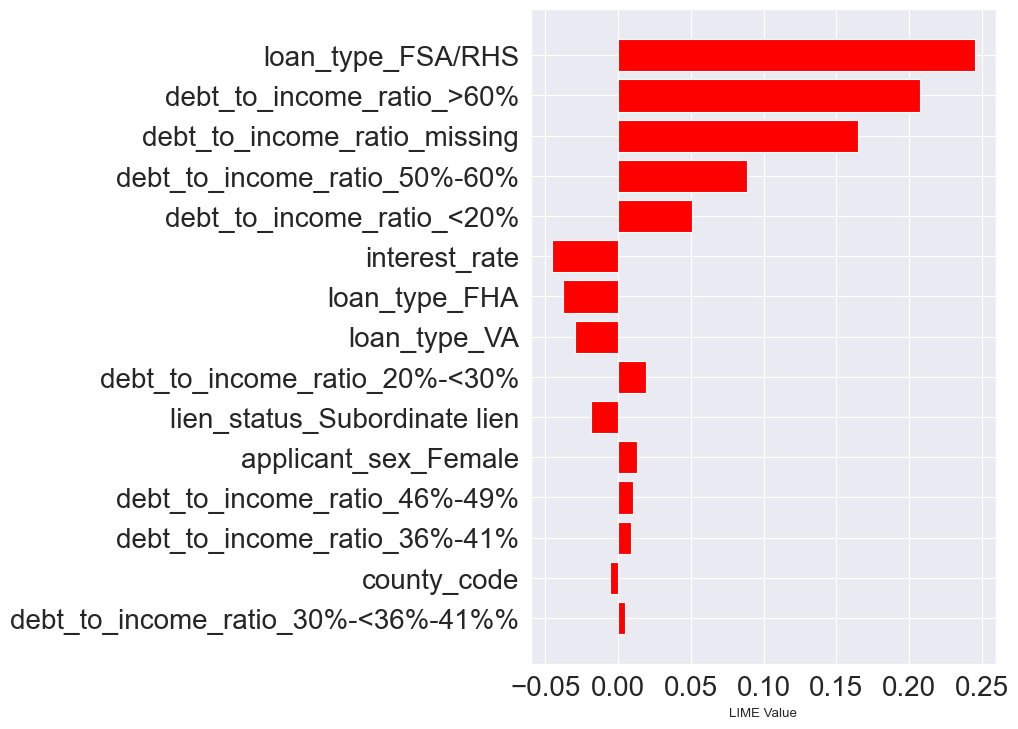
\includegraphics[width=\textwidth,height=5cm,keepaspectratio]{images/CHXX_UPDATE_LIME_individual.png}
        \caption{LIME individual explanations}
        \label{fig:LIME_explanations}
    \end{minipage}
    \caption*{Directly comparing LIME and SHAP explanations for the first 150 observations of the test set: While \textit{debt\_to\_income\_ratio} is an important factor in both explanations, its actual impact varies, as LIME also considers the \textit{loan\_type} feature to be of high importance. Default plotting options were kept: SHAP values are displayed as absolutes, while LIME values show the direction of their impact.}
\end{figure}

While the overall trends are similar with both algorithms, the actual impact of the features varies significantly. While this is not a direct threat to the quality of the results of this thesis, it is a reminder that Explainability algorithms need to be analyzed carefully. 
This ties with the findings of Krishna et al. \parencite{Krishna2022}, who emphasize the importance of understanding the underlying assumptions of Explainability algorithms and the need for a more comprehensive evaluation of their results.

To validate the results of the local explanations, a \textit{Global Surrogate Model} was used. \textbf{figure \ref{fig:Global_Surrogate}} shows the results of the global surrogate model. Specifically, the five most important features according to the global surrogate model are compared to the SHAP and LIME explanations in terms of their relative performance.
It is apparent that the overall trends of SHAP and LIME are close to the global explanations.

\begin{figure}[h]
    \centering
    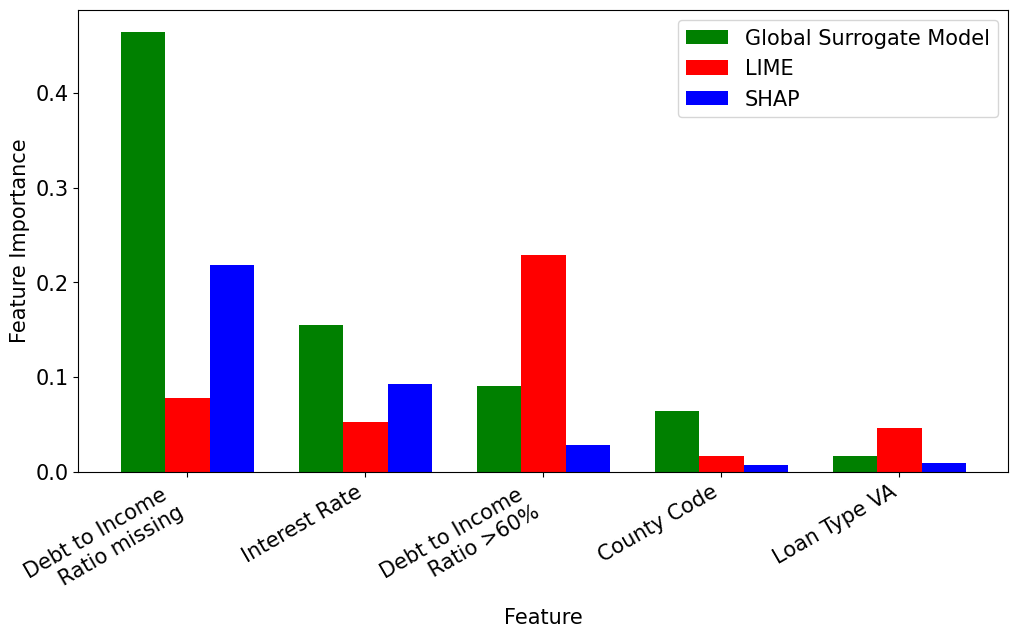
\includegraphics[width=0.85\textwidth]{images/CHXX_UPDATE_Surrogate_SHAP_LIME_combined.png}
    \caption{Global Surrogate Model compared to SHAP and LIME}
    \caption*{Analyzing the 5 most important features according to the global surrogate model implies that the overall trends of SHAP and LIME are close to the global explanations.}
    \label{fig:Global_Surrogate}
\end{figure}

\textbf{Performance}

Even without directly comparable benchmarks available (see \textbf{chapter \ref{subsec:Performance_Assessment}}), the initial model performance can be considered as good. Details can be found in \textbf{table \ref{tab:initial_model_performance_results_1}}.

\begin{table}[h]
    \centering
    \begin{tabular}{l c}
    \toprule
    \textbf{Metric} & \textbf{Value} \\
    \midrule
    \textbf{accuracy} & 0.90 \\
    \textbf{precision} & 0.88 \\
    \textbf{recall} & 0.96 \\
    \textbf{f1} & 0.92 \\
    \textbf{roc\_auc} & 0.94 \\
    \bottomrule
    \end{tabular}
    \caption{Metrics \#1: Initial Model}
    \caption*{The initial model shows a high accuracy and recall, but a lower precision and f1 score. The overall performance can be considered good.}
    \label{tab:initial_model_performance_results_1}
\end{table}

\textbf{Fairness}

\textbf{Table \ref{tab:initial_model_fairness_results_1}} shows the results of the fairness assessment of the initial model. The disparities in the true positive rate and false positive rate are relatively low, while the disparities in the true negative rate and false negative rate are higher.

\begin{table}[h]
    \caption{Metrics \#2: Initial Model}
    \begin{minipage}[t]{0.5\textwidth}
    \centering
    \begin{tabular}{lr}
    \toprule
    \textbf{Metric} & \textbf{Value} \\
    \midrule
    \textbf{Accuracy White} & 0.91 \\
    \textbf{Precision White} & 0.89 \\
    \textbf{Recall White} & 0.97 \\
    \textbf{F1 Score White} & 0.93 \\
    \textbf{AUC White} & 0.94 \\
    \textbf{Accuracy Black} & 0.89 \\
    \textbf{Precision Black} & 0.84 \\
    \textbf{Recall Black} & 0.92 \\
    \textbf{F1 Score Black} & 0.88 \\
    \textbf{AUC Black} & 0.95 \\
    \bottomrule
    \end{tabular}
    \end{minipage}\hfill
    \begin{minipage}[t]{0.5\textwidth}
    \centering
    \begin{tabular}{lr}
    \toprule
    \textbf{Metric} & \textbf{Value} \\
    \midrule
    \textbf{tpr\_disparity} & 0.95 \\
    \textbf{fpr\_disparity} & 0.77 \\
    \textbf{tnr\_disparity} & 1.05 \\
    \textbf{fnr\_disparity} & 2.51 \\
    \bottomrule
    \end{tabular}
    \end{minipage}
    \label{tab:initial_model_fairness_results_1}
    \caption*{The initial model shows a higher accuracy and recall for White applicants, but a higher precision and F1 score for Black applicants. The AUC is higher for Black applicants. The disparities in the true positive rate and false positive rate are relatively low, while the disparities in the true negative rate and false negative rate are higher.}
\end{table}

\subsection{Results of the Iterations}\label{subsec:Iterations}

None of the techniques applied in the iterations led to a significant increase in fairness. The \textit{reweighing} technique managed to improve the overall fairness of the model, but the other techniques did not manage to reach the same level of fairness. 
Figures \textbf{\ref{fig:Initial_Disparity}} to \textbf{\ref{fig:Calibrated_EqOdds_Disparity}} show that the disparity in loan grants between \textit{White} and \textit{Black or African American} applicants was not substantially reduced by any of the iterations, with the calibrated equalized odds algorithm even increasing the disparity.

\begin{figure}[h]
    \centering
    \begin{minipage}{0.5\textwidth}
        \centering
        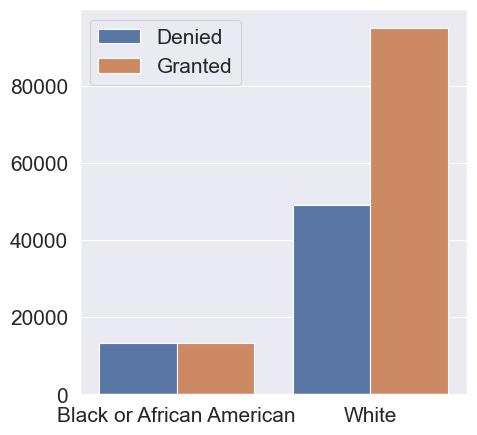
\includegraphics[width=\textwidth]{images/loan_grants_by_protected_attributes/initial.png}
        \caption{Initial Model Disparity}
        \label{fig:Initial_Disparity}
    \end{minipage}\hfill
    \begin{minipage}{0.5\textwidth}
        \centering
        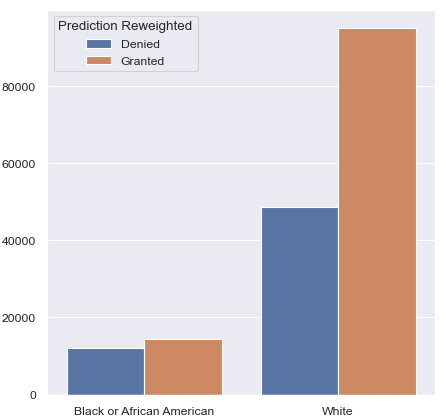
\includegraphics[width=\textwidth]{images/loan_grants_by_protected_attributes/reweighted.png}
        \caption{Reweighed Model Disparity}
        \label{fig:Reweighed_Disparity}
    \end{minipage}
    
    \vspace{1em} 
    
    \begin{minipage}{0.5\textwidth}
        \centering
        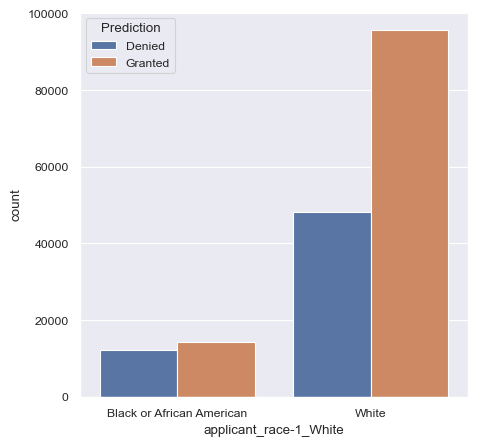
\includegraphics[width=\textwidth]{images/loan_grants_by_protected_attributes/correlation_removed.png}
        \caption{Corr. Rem. Model Disparity}
        \label{fig:Correlation_Removed_Disparity}
    \end{minipage}\hfill
    \begin{minipage}{0.5\textwidth}
        \centering
        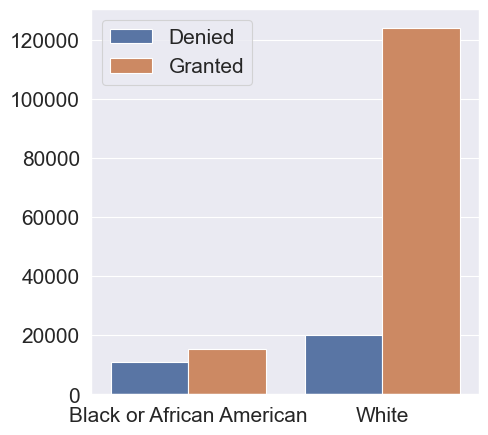
\includegraphics[width=\textwidth]{images/loan_grants_by_protected_attributes/calibrated_eqodds.png} 
        \caption{Cal. Eq. Odds Model Disparity}
        \label{fig:Calibrated_EqOdds_Disparity}
    \end{minipage}
    
    \label{fig:Racial_Disparities}
    \caption*{Apart from the Calibrated Equalized Odds model, which exhibits a higher amount of overall predicted grants, none of the iterations were able to substantially reduce the disparity in granted loans between races.}
\end{figure}

In terms of \textbf{performance}, the iterations did not lead to a significant increase in performance, with the \textit{Calibrated Equalized Odds} model even showing a significant decrease in performance. \textbf{Table \ref{tab:metrics_1_iterations}} shows the results of the performance assessment of the iterations.
All iterations tended to be closer to each other than expected. The best value (which is marked in bold), was only achieved at the third or fourth digit after the comma in many cases, leading to changes in the "best" model across different iterations.

\begin{table}[h]
    \centering
    \caption{Metrics \#1: Iterations}
    \begin{tabular}{l *{4}{>{$}c<{$}}}
    \toprule
    & \textbf{Initial Model} & \textbf{Reweighing} & \textbf{Calibrated Equalized Odds} & \textbf{Correlation Removal} \\
    \midrule
    \textbf{accuracy} & 0.90 & 0.90 & 0.73 & \textbf{0.91} \\
    \textbf{precision} & 0.88 & 0.88 & 0.69 & \textbf{0.88} \\
    \textbf{recall} & 0.96 & \textbf{0.97} & 0.97 & 0.97 \\
    \textbf{f1} & 0.92 & 0.92 & 0.81 & \textbf{0.92} \\
    \textbf{roc\_auc} & \textbf{0.94} & 0.94 & \text{NA} & \text{NA} \\
    \bottomrule
    \end{tabular}
    \caption*{Except the Calibrated Equalized Odds Model, all iterations show a similar performance to the initial model. The Correlation Removal Model shows a slightly higher accuracy and f1 score.}
    \label{tab:metrics_1_iterations}
\end{table}

Similarly to the performance, the iterations did not lead to a significant increase in (subgroup) fairness. The \textit{reweighing} technique managed to improve the overall fairness of the model, but the other techniques did not manage to reach the same level of fairness. \textbf{Table \ref{tab:metrics_2_1_iterations}} shows the results of the fairness assessment of the iterations for the first part of \textit{metrics \#2}.

\begin{table}[h]
    \centering
    \caption{Metrics \#2 (1): Iterations}
    \begin{tabular}{l *{4}{>{$}c<{$}}}
    \toprule
    & \textbf{Initial Model} & \textbf{Reweighing} & \textbf{Calibrated Equalized Odds} & \textbf{Correlation Removal} \\
    \midrule
    \textbf{Accuracy White} & 0.91 & 0.91 & 0.72 & \textbf{0.91} \\
    \textbf{Precision White} & \textbf{0.89} & 0.89 & 0.68 & 0.89 \\
    \textbf{Recall White} & 0.97 & 0.97 & \textbf{0.98} & 0.98 \\
    \textbf{F1 Score White} & 0.93 & 0.92 & 0.81 & \textbf{0.93} \\
    \textbf{AUC White} & \textbf{0.94} & 0.94 & \text{NA} & \text{NA} \\
    \midrule
    \textbf{Accuracy Black} & \textbf{0.89} & 0.88 & 0.81 & 0.88 \\
    \textbf{Precision Black} & 0.84 & 0.81 & 0.73 & \textbf{0.85} \\
    \textbf{Recall Black} & 0.92 & \textbf{0.97} & 0.93 & 0.92 \\
    \textbf{F1 Score Black} & 0.88 & \textbf{0.88} & 0.82 & 0.88 \\
    \textbf{AUC Black} & 0.95 & \textbf{0.95} & \text{NA} & \text{NA} \\
    \bottomrule
    \end{tabular}
    \caption*{Once again, the Calibrated Equalized Odds Model shows a significant decrease in performance. The other models show a similar performance to the initial model.}
    \label{tab:metrics_2_1_iterations}
\end{table}

In terms of disparities (see \textbf{table \ref{tab:metrics_2_2_iterations}}), the \textit{reweighing} technique managed to improve the overall fairness of the model, but the other techniques did not manage to reach the level of the initial model.
While across different model runs the disparities for the iterated models were very comparable, with the \textit{reweighing} technique consistently outperformung the other iterations, the performance in terms of disparities of the initial model varied strongly across different runs.

\begin{table}[h]
    \centering
    \caption{Metrics \#2 (2): Iterations}
    \begin{tabular}{l *{4}{>{$}c<{$}}}
    \toprule
    & \textbf{Initial Model} & \textbf{Reweighing} & \textbf{Calibrated Equalized Odds} & \textbf{Correlation Removal} \\
    \midrule
    \textbf{tpr\_disparity} & 0.95 & \textbf{1.00} & 0.95 & 0.94 \\
    \textbf{fpr\_disparity} & 0.77 & \textbf{1.00} & 0.43 & 0.76 \\
    \textbf{tnr\_disparity} & 1.01 & \textbf{1.00} & 2.23 & 1.06 \\
    \textbf{fnr\_disparity} & 2.51 & \textbf{0.84} & 3.25 & 3.42 \\
    \bottomrule
    \end{tabular}
    \caption*{In terms of disparities, the positive effects of reweighing show, with the algorithm outperforming the other iterations.}
    \label{tab:metrics_2_2_iterations}
\end{table}

Visualizing the results of the iterations in a comparison chart (\textbf{figure \ref{fig:Fairness_Comparison_Chart}}) shows that while the initial model managed to put out values with a comparably high fairness as measured by disparities, reweighing managed to improve this overall performance. The other two models however did not manage to reach the same level of fairness.

\begin{figure}
    \centering
    \caption{Fairness Comparison Chart}
    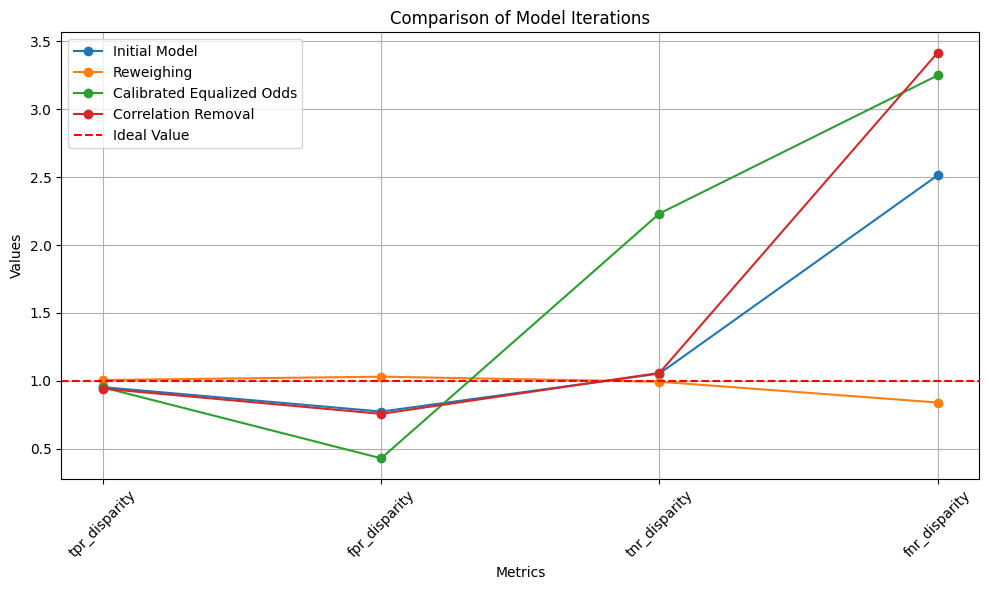
\includegraphics[width=0.85\textwidth]{images/CHXX_UPDATE_Results_Line.png}
    \caption*{While the initial model managed to put out values with a comparably high fairness as measured by disparities, reweighing managed to improve this overall performance. The other two models however did not manage to reach the same level of fairness.}
    \label{fig:Fairness_Comparison_Chart}
\end{figure}

% \section{Limitations}\label{sec:Limitations} - hier oder am Ende?

\section{Results}\label{sec:Results}

\subsection{Mortgage Classifier (Benchmark)}\label{subsec:Mortgage Classifier (Benchmark) Results}

In order to assess whether a predictive algorithm would pick up on and reproduce bias in the data, an initial classification model (as described in \textbf{chapter \ref{subsec:Model_Training_and_Prediction}} and detailed in \textbf{table \ref{tab:CH03_Model_Details}}) was trained on the HMDA dataset (see \textbf{chapter \ref{subsec:HMDA_Data}}) with the goal of predicting whether a mortgage would be granted or not for a given applicant.
The results of this model were assessed in terms of performance and fairness.

\textbf{Performance Assessment}

When fitting the neural network to the training data, the \textit{training accuracy} of the model improved rapidly initially, leveling off after a few epochs. The \textit{validation accuracy} started at a high level and constantly improved by small increments, suggesting that both the model learning process as well as the ability to generalize to previously unseen data were successful. 
The training process was stopped by an early\_stopping callback, with the ninth epoch being the one with the least validation loss. The training results of the best epoch were:
\begin{itemize}
    \item \textit{Training Accuracy}: 0.90
    \item \textit{Validation Accuracy}: 0.90
    \item \textit{Training Loss}: 0.28
    \item \textit{Validation Loss}: 0.28
\end{itemize}
The history of the training process is depicted in \textbf{figure \ref{fig:Model_Training_History}}.

\begin{figure}
    \centering
    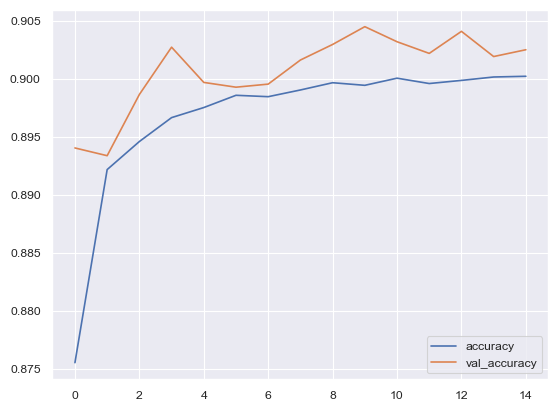
\includegraphics[width=0.85\textwidth]{images/Model_Training/Initial_Training_History.png}
    \caption{Training History of the Mortgage Classifier Model}
    \medskip
    \small
    The training history of the initial mortgage classifier model, showing the training and validation accuracy and loss over the course of the training process. The training accuracy improved constantly until the early\_stopping callback. The validation accuracy constantly improved, suggesting a successful learning process.
    \label{fig:Model_Training_History}
\end{figure}

The model was then evaluated on the test dataset, which was not seen by the model during training. The results of the performance evaluation (i.e. \textit{metrics \#1}) are shown in \textbf{table \ref{tab:Model_Evaluation}}. The model achieved an \textit{accuracy} of 0.90, a \textit{precision} of 0.88, a \textit{recall} of 0.97, and an \textit{F1-score} of 0.92. 
As stated in \textbf{chapter \ref{subsec:Model_Training_and_Prediction}}, the original model output were probabilities between 0 and 1. These could be used to calculate ROC AUC and plot the corresponding ROC curve, which can be seen in \textbf{figure \ref{fig:Model_Training_ROC}}. The \textit{ROC-AUC} score was 0.94, indicating a high level of model performance. 
Converting the probabilities into predictions with a threshold of 0.5 fulfilled the classification requirement. The \textit{confusion matrix} is depicted in \textbf{figure \ref{fig:Model_Confusion_Matrix}}. The model managed to achieve a high number of true positives and true negatives, while the number of false negatives was low. However, the number of false positives was nearly 8\% of all predictions.

\begin{table}[!htbp]
    \centering
    \begin{tabular}{l c}
    \toprule
    \textbf{Metric} & \textbf{Value} \\
    \midrule
    \textbf{accuracy} & 0.90 \\
    \textbf{precision} & 0.88 \\
    \textbf{recall} & 0.97 \\
    \textbf{f1} & 0.92 \\
    \bottomrule
    \end{tabular}
    \caption{Metrics \#1: Initial Model}
    \small
    The mortgage classifier model was evaluated on the test dataset, achieving an accuracy of 0.90, a precision of 0.88, a recall of 0.97, and an F1-score of 0.92.
    \label{tab:Model_Evaluation}
\end{table}

\begin{figure}
    \centering
    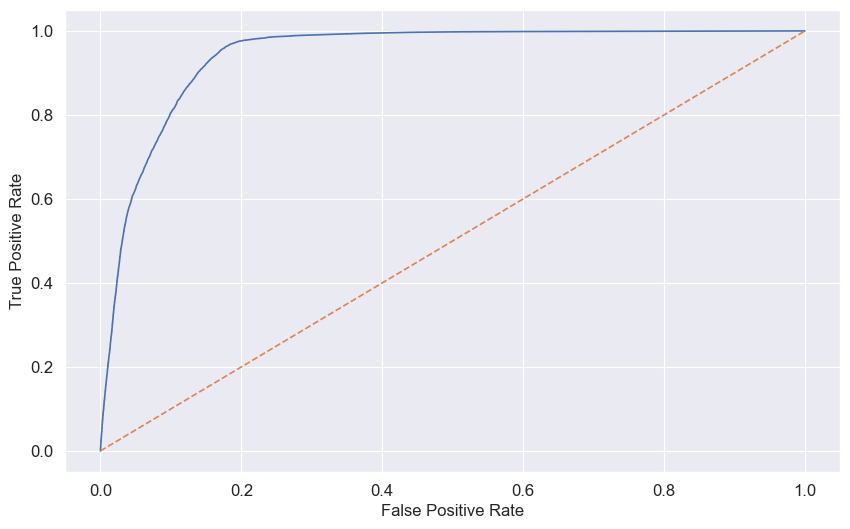
\includegraphics[width=0.85\textwidth]{images/Model_Training/Initial_ROC_curve.png}
    \caption{ROC curve of the Mortgage Classifier Model}
    \medskip
    \small
    The ROC curve is significantly above the diagonal baseline, indicating high predictive performance.
    \label{fig:Model_Training_ROC}
\end{figure}

\begin{figure}
    \centering
    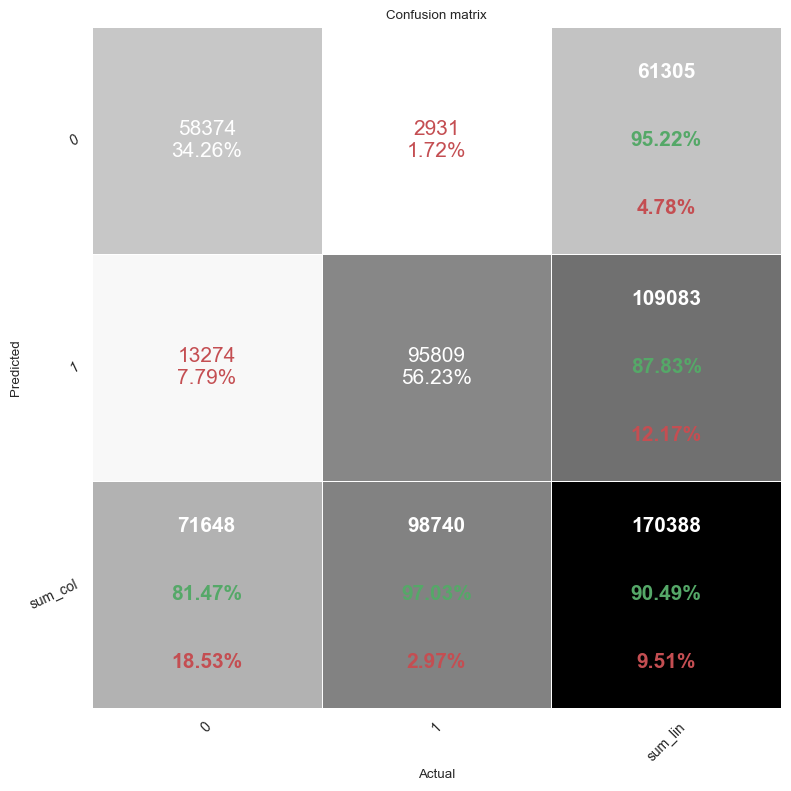
\includegraphics[width=0.85\textwidth]{images/Model_Training/Initial_Confusion_Matrix.png}
    \caption{Confusion Matrix on the Test Dataset of the Mortgage Classifier Model}
    \medskip
    \small
    The confusion matrix of the mortgage classifier model on the test dataset. The model achieved a high number of true positives and true negatives. The number of false negatives was low, however, false positives made up nearly 8\% of all predictions.
    \label{fig:Model_Confusion_Matrix}
\end{figure}

\textbf{Fairness Assessment}

Following the research question (see \textbf{chapter \ref{ch:Introduction}}), the \textit{detection of unfairness} in the predictions is an explicit goal of this thesis. To address this, the fairness assessment outlined in \textbf{chapter \ref{subsec:Model_Training_and_Prediction}} was applied to the predictions. The results of the fairness assessment (i.e. \textit{metrics \#2}) are shown in \textbf{table \ref{tab:Fairness_Assessment_Initial}}. 
The model performed slightly better for \textit{White} applicants than for \textit{Black} applicants. The \textit{accuracy} for \textit{White} applicants was 0.91, while it was 0.88 for \textit{Black} applicants. The \textit{precision} for \textit{White} applicants was 0.89, while it was 0.82 for \textit{Black} applicants. The \textit{recall} for \textit{White} applicants was 0.97, while it was 0.96 for \textit{Black} applicants. 
The \textit{F1-score} for \textit{White} applicants was 0.93, while it was 0.88 for \textit{Black} applicants. The \textit{AUC} for \textit{White} applicants was 0.94, while it was 0.95 for \textit{Black} applicants. 
In terms of disparities (where the optimal value is \textbf{1}), the model performed comparably well in all disciplines except the \textit{fnr\_disparity}, which was 1.42. This indicates that the model was more likely to predict a false negative for \textit{Black} applicants than for \textit{White} applicants.

\begin{table}[!htbp]
    \centering
    \begin{tabular}{lr}
    \toprule
    \textbf{Metric} & \textbf{Value} \\
    \midrule
    \textbf{Accuracy White} & 0.91 \\
    \textbf{Precision White} & 0.89 \\
    \textbf{Recall White} & 0.97 \\
    \textbf{F1 Score White} & 0.93 \\
    \textbf{AUC White} & 0.94 \\
    \midrule
    \textbf{Accuracy Black} & 0.88 \\
    \textbf{Precision Black} & 0.82 \\
    \textbf{Recall Black} & 0.96 \\
    \textbf{F1 Score Black} & 0.88 \\
    \textbf{AUC Black} & 0.95 \\
    \midrule
    \textbf{tpr\_disparity} & 0.99 \\
    \textbf{fpr\_disparity} & 0.96 \\
    \textbf{tnr\_disparity} & 1.01 \\
    \textbf{fnr\_disparity} & 1.42 \\
    \bottomrule
    \end{tabular}
    \caption{Metrics \#2: Initial Model}
    \label{tab:Fairness_Assessment_Initial}
    \small
    The benchmark model showed a slightly better performance for \textit{White} applicants than for \textit{Black} applicants. The disparities were comparably low, except for the \textit{fnr\_disparity}, which was 1.42.
\end{table}

\subsection{Explainability}\label{Explainability Results}

As stated in \textbf{chapter \ref{subsec:Explainability}}, three different approaches to explainability were utilized not only to support the analysis of fairness by providing insights into the model's decision-making process, but also to provide a better understanding of the model's behavior: \textit{SHAP}, \textit{LIME}, and a \textit{Global Surrogate Model}. 

\textbf{SHAP}

As stated in \textbf{chapter \ref{subsec:algorithms}}, the SHAP algorithm tries to game-theoretically distribute the value of the final prediction among the individual features considered.
\textbf{Figure \ref{fig:SHAP_beeswarm}} shows the SHAP beeswarm plot, which displays the distribution of the SHAP values for each feature in the dataset. The color indicates the feature value (red = higher; blue = lower), while the x-axis shows the SHAP value (left of center = negative; right of center = positive). The y-axis shows the feature name. The plot includes 150 values from the SHAP values of the test dataset.
It showed that the most influential features according to SHAP were \textit{debt\_to\_income\_ratio\_missing, interest\_rate, loan\_to\_value\_ratio}, and \textit{debt\_to\_income\_ratio\_>60\%}.
While it was apparent how missingness in the debt to income ratio (missingness is negative, availability is positive) and values >60\% in the debt to income ratio (higher is negative, lower is positive) affected the model decision, interest rates and the loan-to-value-ratios as the numerical variables were less intuitive to interpret.
Although most medium to high interest rates seemed to be related with slight negative impacts, there also was a cluster of higher values for these variables corresponding with positive prediction influences.
As all other variables were categorical, their interpretations were straightforward. Albeit their absolute impact in terms of SHAP values was limited, it is noteworthy that the \textit{protected variables} of race and sex were in fact picked up on by the model.
In every case where a decision was negatively influenced by the \textit{race} of the applicant, the applicant in question was Black or African American (as can be inferred from all values left of the center of the x-axis for \textit{applicant\_race-1\_White} being colored blue for this feature, meaning a lower value, which in turn means Black or African American ethnicity).
A similar picture was observed for the \textit{sex} of the applicant: In most cases where the model picked up on the sex being an influential factor on the model decision, the applicant in question was \textit{female} and vice versa.

\begin{figure}[!htbp]
    \centering
    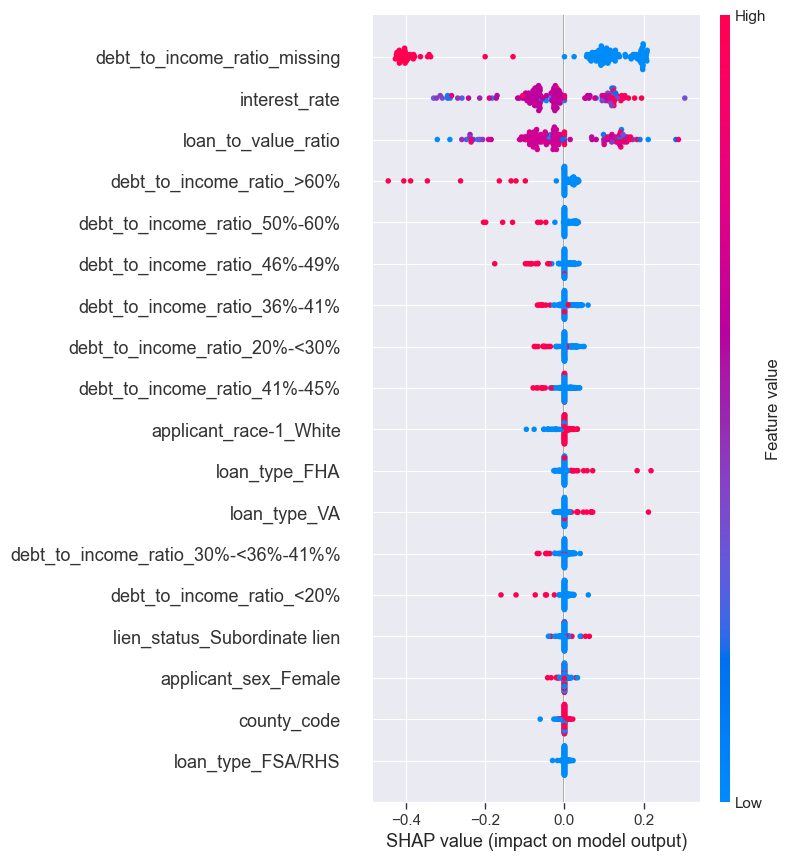
\includegraphics[width=0.85\textwidth]{images/SHAP_Individual_Analyses/beeswarm.png}
    \caption{SHAP beeswarm plot}
    \medskip
    \small
    The SHAP beeswarm plot shows the distribution of the SHAP values for each feature in the dataset. The color indicates the feature value, while the x-axis shows the SHAP value. The y-axis shows the feature name.
    \label{fig:SHAP_beeswarm}
\end{figure}

The \textit{expected value} of the SHAP values (i.e. the baseline before consideration of any feature importance) was \textit{0.57}. This corresponds to the imbalance in the original HMDA data (see \textbf{chapter \ref{fig:CHXX_Target_Variable_Distribution}}).
\textbf{Figure \ref{fig:SHAP_Individual_Analyses}} shows the SHAP values for four selected applicants. The force plots displayed show how the individual values of the features influence the model's decision according to SHAP. 
Each individual prediction results from the aforementioned \textit{expected value} and the sum of inferred importances of the features (exemplarily, in the first plot displayed in \textbf{figure \ref{fig:SHAP_Individual_Analyses}}, the feature importances amount to roughly positive 0.4, leading to a total value of 0.97 and therefore a positive prediction, i.e. a granted mortgage).
It shows that SHAP attributes a high importance to (missingness of) the Debt to income ratio. Due to the values being scaled, a value of \textit{-0.59} corresponds to \textit{debt\_to\_income\_ratio\_missing == False} and a value of \textit{1.68} corresponds to \textit{debt\_to\_income\_ratio\_missing == True}. Therefore, SHAP considers missingness in this variable as negative and availability as positive.
Considering the last applicant displayed (\textit{Black or African American Male, Debt to Income Ratio available}), it does however show that even availabilty of the Debt to Income Ratio does not guarantee a positive model decision.
According to SHAP, none of the decisions displayed here (and in the whole set of predictions in general) were significantly informed by any protected attribute. However, confounding factors might still be present, as the model might have learned to discriminate based on other features that are correlated with the protected attributes.

\begin{figure}[!htbp]
    \centering
    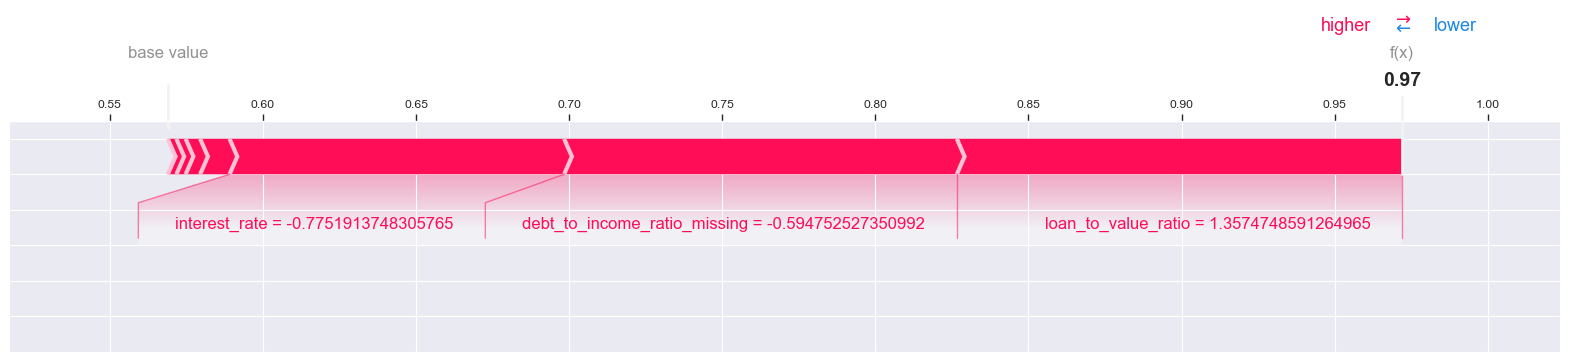
\includegraphics[width=0.95\textwidth]{images/SHAP_Individual_Analyses/SHAP_individual_0.png}
    \small
    White Male, Debt to Income Ratio available
    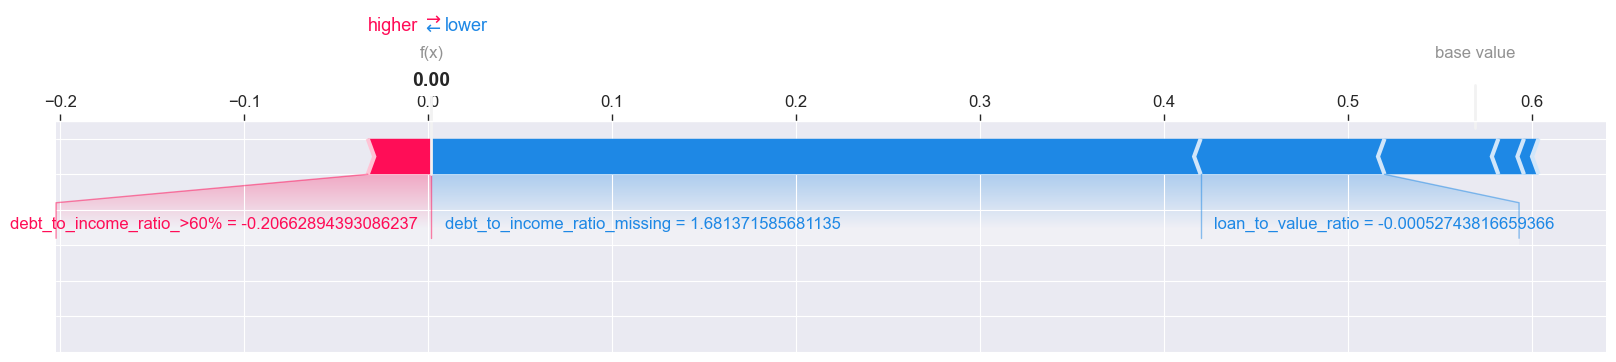
\includegraphics[width=0.95\textwidth]{images/SHAP_Individual_Analyses/SHAP_individual_1.png}
    \small
    White Male, Debt to Income Ratio missing
    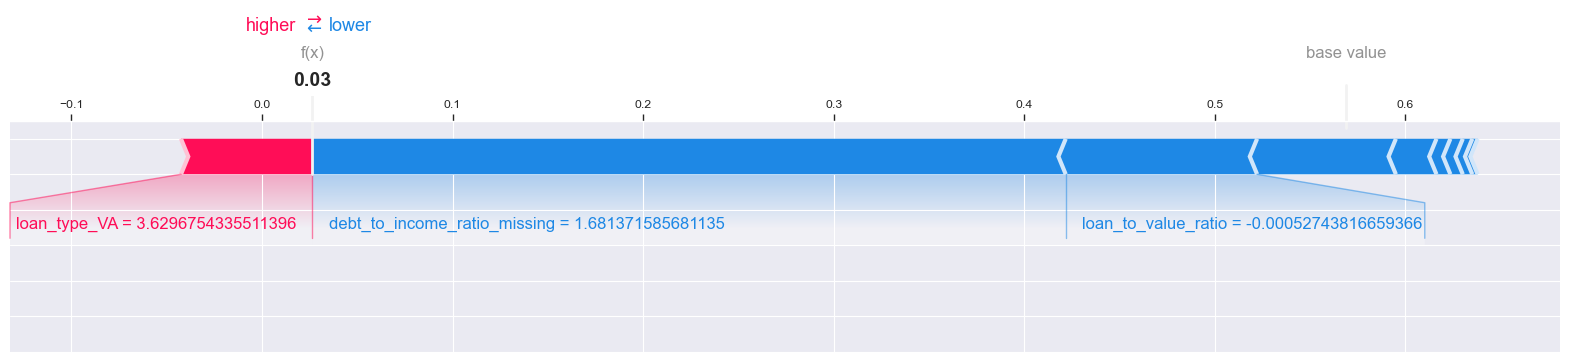
\includegraphics[width=0.95\textwidth]{images/SHAP_Individual_Analyses/SHAP_individual_21.png}
    \small
    Black or African American Male, Debt to Income Ratio missing
    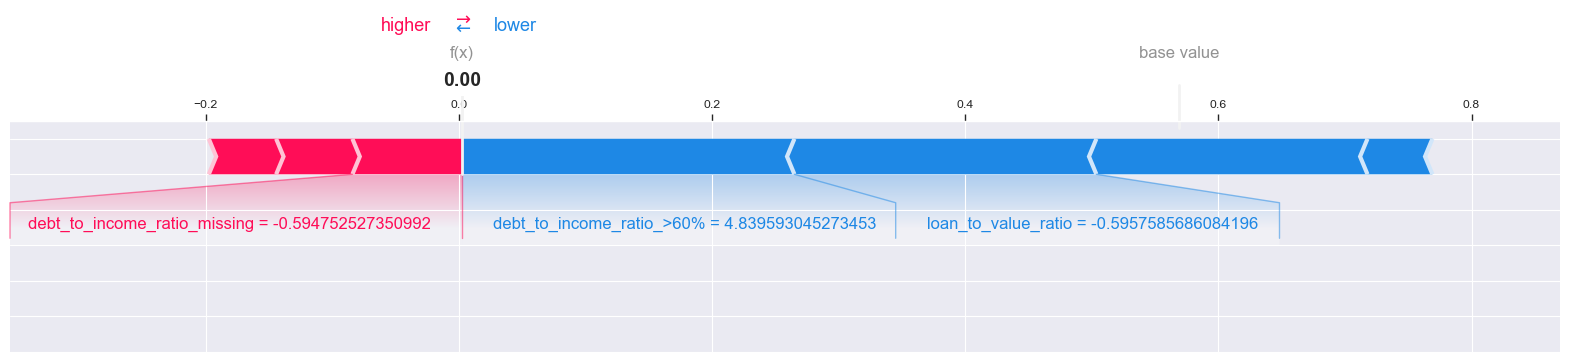
\includegraphics[width=0.95\textwidth]{images/SHAP_Individual_Analyses/SHAP_individual_139.png}
    \small
    Black or African American Male, Debt to Income Ratio available
    \caption{Selected SHAP Individual Analyses}
    \medskip
    \small
    Comparing four selected Male applicants with different characteristics shows that, in general, SHAP attributes a high importance to (missingness of) the Debt to Income Ratio. However, it is not the sole decision criterion, as the last applicant displayed shows.
    \label{fig:SHAP_Individual_Analyses}
\end{figure}

\textbf{LIME}

The LIME algorithm, in contrast to SHAP, tries to explain the model's decision on a local level by approximating the model's behavior around a single prediction (see \textbf{chapter \ref{subsec:algorithms}}).
\textbf{Figure \ref{fig:LIME_Individual_Analyses}} shows the LIME individual feature importance plot for a selected applicant, specifically the same applicant that is denoted as \textit{White Male, Debt to Income Ratio available} in \textbf{figure \ref{fig:SHAP_Individual_Analyses}}. The x-axis shows the feature importance, while the y-axis shows the feature name.
It showed that LIME attributes a high importance to the \textit{loan type} and the \textit{debt to income ratio}. Once again, the \textit{protected attributes} had very little absolute influence on the model's decision according to LIME.

\begin{figure}[!htbp]
    \centering
    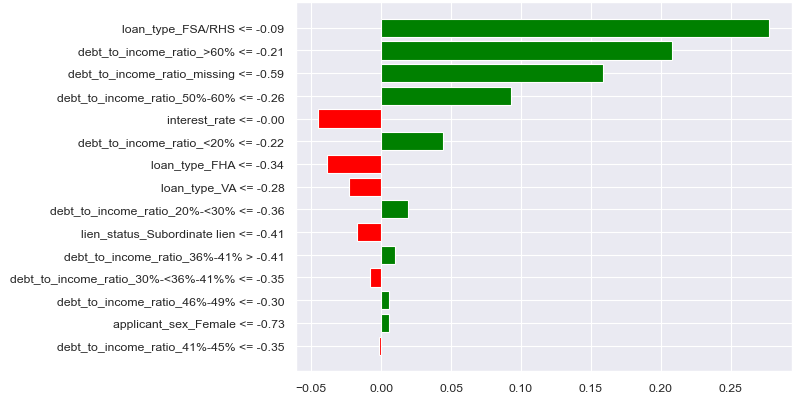
\includegraphics[width=0.85\textwidth]{images/CHXX_LIME_individual.png}
    \caption{LIME Individual Feature Importance}
    \medskip
    \small
    The LIME individual feature importance plot shows the direction and the impact of the features on the model's decision for a selected applicant. The x-axis shows the feature importance, while the y-axis shows the feature name.
    \label{fig:LIME_Individual_Analyses}
\end{figure}

While the overall explanations on which features are influential are similar for both SHAP and LIME, the actual impact of the features varies significantly. While this is not a direct threat to the quality of the results of this thesis, it is a reminder that explainability algorithms need to be analyzed carefully. 
This ties with the findings of Krishna et al. \parencite{Krishna2022}, who emphasize the importance of understanding the underlying assumptions of explainability algorithms and the need for a more comprehensive evaluation of their results.

\textbf{Global Surrogate Model}

To validate the results of the local explanations, a \textit{Global Surrogate Model} was used. \textbf{figure \ref{fig:Global_Surrogate}} shows the results of the global surrogate model. Specifically, the five most important features according to the global surrogate model are compared to the SHAP and LIME explanations in terms of their relative performance.
It showed that all three explanation algorithms mainly agree on the three most important features in the data (\textit{debt\_to\_income\_ratio\_missing, interest\_rate}, and \textit{debt\_to\_income\_ratio\_>60\%}), although LIME attributes a different order of importance to them compared to SHAP and the global surrogate model.

\begin{figure}[!htbp]
    \centering
    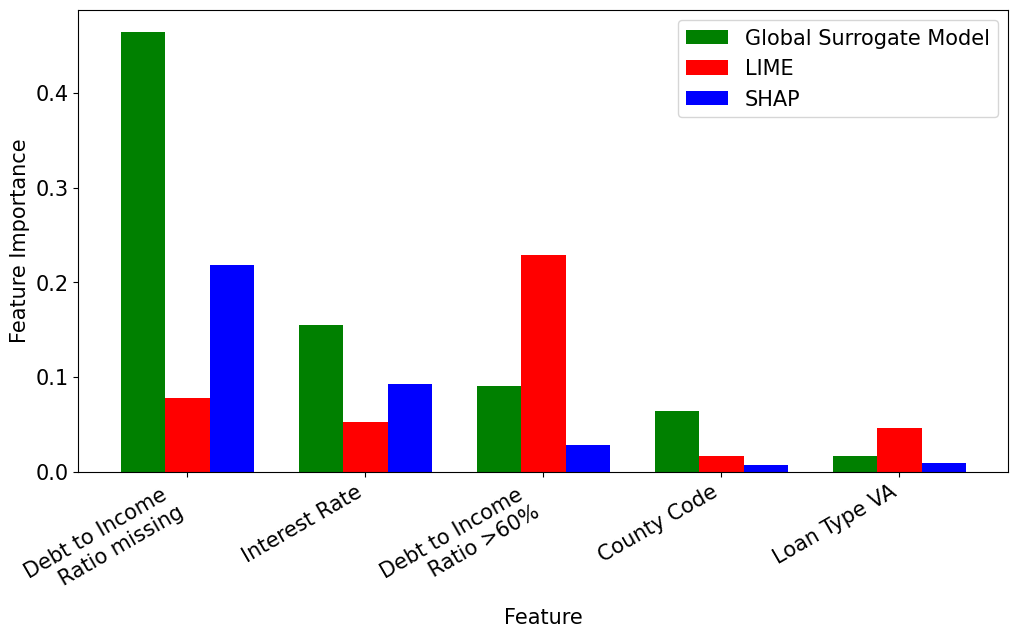
\includegraphics[width=0.85\textwidth]{images/CHXX_UPDATE_Surrogate_SHAP_LIME_combined.png}
    \caption{Global Surrogate Model compared to SHAP and LIME}
    \medskip
    \small
    Analyzing the 5 most important features according to the global surrogate model implies that the overall trends of SHAP and LIME are close to the global explanations.
    \label{fig:Global_Surrogate}
\end{figure}

\subsection{Fairness Adjustments}\label{Fairness Adjustments Results}

While the performance of the benchmark mortgage classifier detailed in \textbf{chapter \ref{subsec:Mortgage Classifier (Benchmark) Results}} was satisfactory, the scope of this thesis (see \textbf{chapter \ref{ch:Introduction}}) included taking an iterative approach to improve fairness without sacrificing predictive performance, as outlined in \textbf{chapter \ref{subsec:Iterations}}.
To this end, the following fairness adjustments were applied to the model: \textit{Reweighing}, \textit{Correlation Remover} and \textit{Calibrated Equalized Odds}. The aim was to reach improvement in at least one of the two metric sets, compared to the benchmark performance depicted in \textbf{table \ref{tab:Model_Evaluation}} (\textit{metrics \#1}) and \textbf{table \ref{tab:Fairness_Assessment_Initial}} (\textit{metrics \#2}).

\textbf{Reweighing}

XXX

\textbf{Correlation Remover}

XXX

\textbf{Calibrated Equalized Odds}

XXX

\textbf{Summary}

Considering the overall \textit{performance} of the different approaches, all models except the \textit{calibrated equalized odds} algorithms performed on a similar, good level (see \textbf{table \ref{tab:metrics_1_iterations_summary}}).
The \textit{correlation removal} algorithm managed to slightly outperform the benchmark model in terms of \textit{accuracy}, \textit{precision}, and \textit{f1-score}, while the \textit{calibrated equalized odds} algorithm managed to slightly outperform the benchmark model in terms of \textit{recall}.

\begin{table}[!htbp]
    \centering
    \begin{tabular}{l *{4}{>{$}c<{$}}}
    \toprule
    & \textbf{Initial Model} & \textbf{Reweighing} & \textbf{Calibrated Equalized Odds} & \textbf{Correlation Removal} \\
    \midrule
    \textbf{accuracy} & 0.90 & 0.90 & 0.73 & \textbf{0.91} \\
    \textbf{precision} & 0.88 & 0.88 & 0.69 & \textbf{0.88} \\
    \textbf{recall} & 0.97 & 0.97 & \textbf{0.97} & 0.97 \\
    \textbf{f1} & 0.92 & 0.92 & 0.81 & \textbf{0.92} \\
    \textbf{roc\_auc} & \textbf{0.94} & 0.94 & \text{NA} & \text{NA} \\
    \bottomrule
    \end{tabular}
    \caption{Metrics \#1: Fairness Adjustments Summary}
    \small
    Results of \textit{metrics \#1} for all applied algorithms. The values are rounded, the highest scores are marked \textbf{bold}.
    \label{tab:metrics_1_iterations_summary}
\end{table}

In terms of \textit{fairness}, no significant optimizations could be achieved. The \textit{reweighing} technique managed to improve the overall fairness of the model, but the other techniques did not manage to reach the same level of fairness. 
\textbf{Figure \ref{fig:Bar_Grant_per_Race}} shows that the differences in loan grants between \textit{White} and \textit{Black or African American} applicants was not substantially reduced by any of the iterations, with the calibrated equalized odds algorithm even increasing the difference.

\begin{figure}[!htbp]
    \centering
    \begin{minipage}{0.5\textwidth}
        \centering
        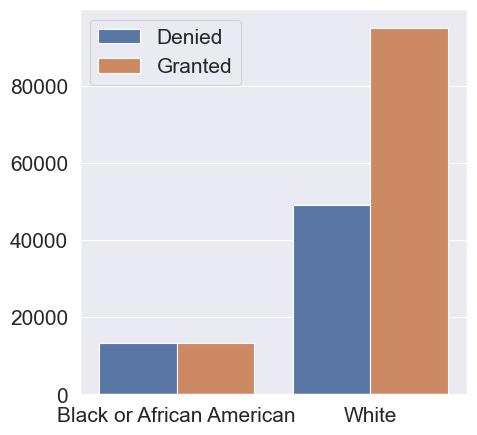
\includegraphics[width=\textwidth]{images/loan_grants_by_protected_attributes/initial.png}
        \small
        Benchmark Model
    \end{minipage}\hfill
    \begin{minipage}{0.5\textwidth}
        \centering
        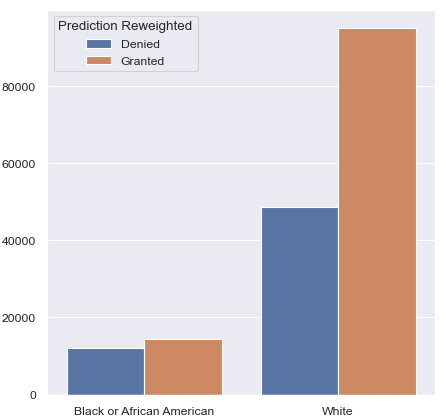
\includegraphics[width=\textwidth]{images/loan_grants_by_protected_attributes/reweighted.png}
        \small
        Reweighing
    \end{minipage}
    
    \begin{minipage}{0.5\textwidth}
        \centering
        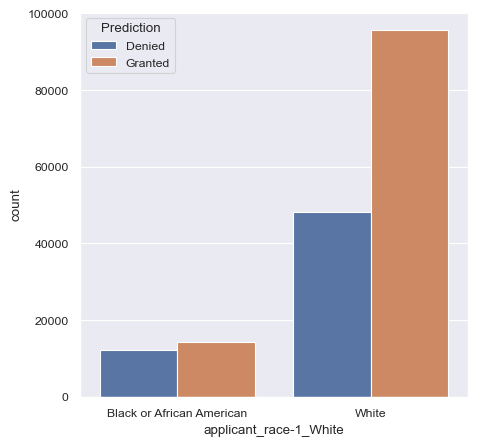
\includegraphics[width=\textwidth]{images/loan_grants_by_protected_attributes/correlation_removed.png}
        \small
        Correlation Removal
    \end{minipage}\hfill
    \begin{minipage}{0.5\textwidth}
        \centering
        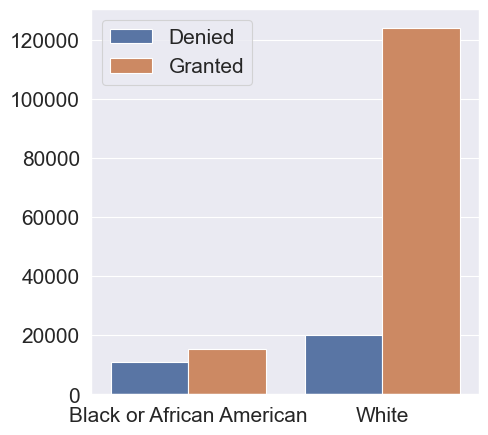
\includegraphics[width=\textwidth]{images/loan_grants_by_protected_attributes/calibrated_eqodds.png} 
        \small
        Calibrated Equalized Odds
    \end{minipage}
    
    \caption{Differences in Positive Predictions per Model}
    \label{fig:Bar_Grant_per_Race}
    \medskip
    \small
    Apart from the Calibrated Equalized Odds model, which exhibits a higher amount of overall predicted grants, none of the iterations were able to substantially reduce the disparity in granted loans between races.
\end{figure}

\textbf{Figure \ref{fig:Fairness_Adjustments_Results_Line}} shows the results of the fairness adjustments in terms of the \textit{disparities} of the model. The disparities were calculated for the \textit{true positive rate}, the \textit{false positive rate}, the \textit{true negative rate}, and the \textit{false negative rate}. 
The disparities were calculated for the \textit{White} and \textit{Black or African American} applicants. As they are relative terms, only the relation of the disparities to the other group is shown.
The disparities were comparably low for the \textit{true positive rate}, while all the other disparities show at least one outlier. The \textit{reweighed} model was the only one that produces satisfactory results in terms of fairness as measured by disparities across all four KPIs, with the benchmark model coming in second.

\begin{figure}[!htbp]
    \centering
    \includegraphics[width=0.85\textwidth]{images/CHXX_Update_Results_Line.png}
    \caption{Fairness Adjustments Results}
    \medskip
    \small
    The results of the fairness adjustments in terms of the disparities of the model. The disparities were calculated for the \textit{true positive rate}, the \textit{false positive rate}, the \textit{true negative rate}, and the \textit{false negative rate}. They were calculated for the \textit{White} and \textit{Black or African American applicants}. Values closer to 1 are better, the gray area represents a good level of fairness.
    \label{fig:Fairness_Adjustments_Results_Line}
\end{figure}

Adding up all fairness metrics for all iterations (see \textbf{table \ref{tab:metrics_2_iterations_summary}}) resulted in a mixed picture.
While the \textit{reweighing} algorithm managed to improve the fairness of the outcomes in terms of disparities (as can also be inferred from \textbf{figure \ref{fig:Fairness_Adjustments_Results_Line}}), the predictive power of the model for subgroups did not show a single optimal model.

\begin{table}[!htbp]
    \centering
    \begin{tabular}{l *{4}{>{$}c<{$}}}
    \toprule
    & \textbf{Initial Model} & \textbf{Reweighing} & \textbf{Calibrated Equalized Odds} & \textbf{Correlation Removal} \\
    \midrule
    \textbf{Accuracy White} & 0.91 & 0.91 & 0.72 & \textbf{0.91} \\
    \textbf{Precision White} & \textbf{0.89} & 0.89 & 0.68 & 0.89 \\
    \textbf{Recall White} & 0.97 & 0.97 & \textbf{0.98} & 0.98 \\
    \textbf{F1 Score White} & 0.93 & 0.93 & 0.81 & \textbf{0.93} \\
    \textbf{AUC White} & \textbf{0.94} & 0.94 & \text{NA} & \text{NA} \\
    \midrule
    \textbf{Accuracy Black} & 0.88 & 0.88 & 0.81 & \textbf{0.89} \\
    \textbf{Precision Black} & 0.82 & 0.81 & 0.73 & \textbf{0.84} \\
    \textbf{Recall Black} & 0.96 & \textbf{0.97} & 0.93 & 0.93 \\
    \textbf{F1 Score Black} & 0.88 & \textbf{0.88} & 0.82 & 0.88 \\
    \textbf{AUC Black} & \textbf{0.95} & 0.95 & \text{NA} & \text{NA} \\
    \midrule
    \textbf{tpr\_disparity} & 0.99 & \textbf{0.99} & 0.95 & 0.96 \\
    \textbf{fpr\_disparity} & 0.96 & \textbf{1.00} & 0.43 & 0.80 \\
    \textbf{tnr\_disparity} & 1.01 & \textbf{1.00} & 2.23 & 1.05 \\
    \textbf{fnr\_disparity} & 1.42 & \textbf{1.20} & 3.25 & 2.67 \\
    \bottomrule
    \end{tabular}
    \caption{Metrics \#2: Fairness Adjustments Summary}
    \small
    Results of \textit{metrics \#2} for all applied algorithms. The values are rounded, the highest scores (respectively those closest to 1 for the disparity calculations) are marked \textbf{bold}.
    \label{tab:metrics_2_iterations_summary}
\end{table}